\section{Deadlock Detection}
\subsection{Determine which lock request will be granted, blocked by the lock manager (LM)}

\begin{figure}
\centering
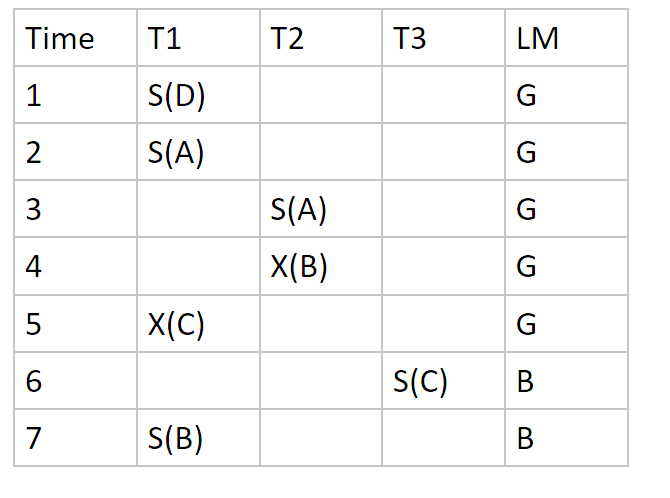
\includegraphics[width=0.7\linewidth]{C:/Users/DennisThinhTan/Documents/GitHub/INDADHandIn4/image/Lm1Table}
\caption[Table showing how LM is handling locks]{Table showing how LM is handling lock requests.}
\label{fig:LmTable}
\end{figure}

\subsection{wait-for graph for the lock requests in the table showed in Figur: \ref{fig:LmTable}}
	
\begin{figure}
\centering
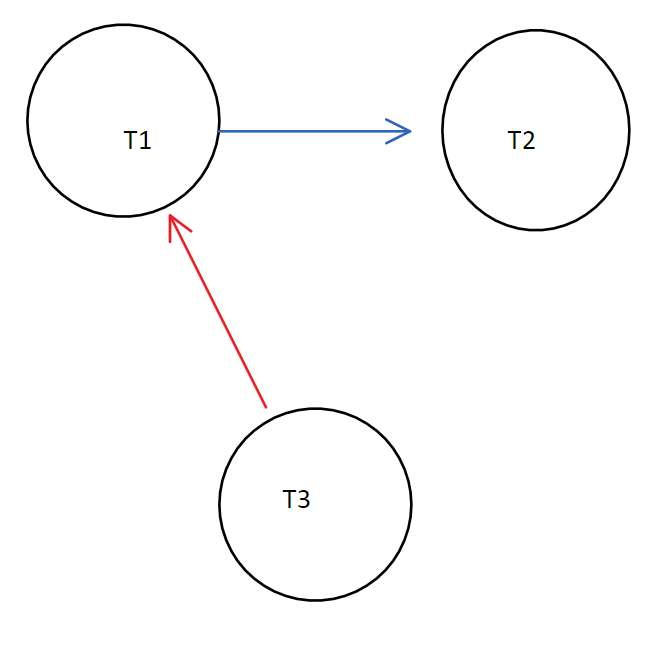
\includegraphics[width=0.7\linewidth]{C:/Users/DennisThinhTan/Documents/GitHub/INDADHandIn4/image/waitForGraphForLM}
\caption[Wait-for graph of LM]{}
\caption{Wait-for graph of LM}
\label{fig:waitForGraphForLM}
\end{figure}

\pagebreak
\subsection{Determine whether there exists a deadlock in the lock requests in the table above and briefly explain why}
There are no deadlock since the wait-for graph (Figur \ref{fig:waitForGraphForLM}) is acyclic.
